\chapter{Introduction}

\section{Motivation}

Even with rapid reduction in costs due to the commercialization of spacecraft components and launch services, all space systems face the unique challenge of being extremely difficult to repair or configure after deployment. Space organizations reduce risk by rigorously testing their designs on the ground all the way from the component to system level. This ability to test flight hardware and software before launch is a crucial part in reducing on-orbit failures. The nature of these tests change as the design of the system matures, with each test placing the system in conditions closer to the operational environment. 

\begin{figure}[h]
    \centering
    \begin{tikzpicture}[
  scale=1.0, % <— master size knob
  every node/.style={transform shape},
  block/.style={
    rectangle, draw, rounded corners,
    fill=blue!10, minimum width=7em, minimum height=3.2em,
    align=center
  },
  line/.style={-Latex, thick},
  node distance=1.3cm and 1.3cm
]

% Nodes
\node[block] (design) {Spacecraft\\Design};
\node[block, right=of design] (sim) {Simulation};
\node[block, right=of sim] (hil) {Hardware-in-the-Loop\\Testing};
\node[block, below=of hil] (ab) {Physical Dynamics\\Simulator};
\node[block, left=of ab] (launch) {Launch};

% Arrows
\draw[line] (design) -- (sim);
\draw[line] (sim) -- (hil);
\draw[line] (hil) -- (ab);
\draw[line] (ab) -- (launch);

\end{tikzpicture}
    \caption{An example spacecraft ADCS testing campaign}
    \label{fig:ADCS_tests}
\end{figure}

\begin{figure}[h]
    \centering
    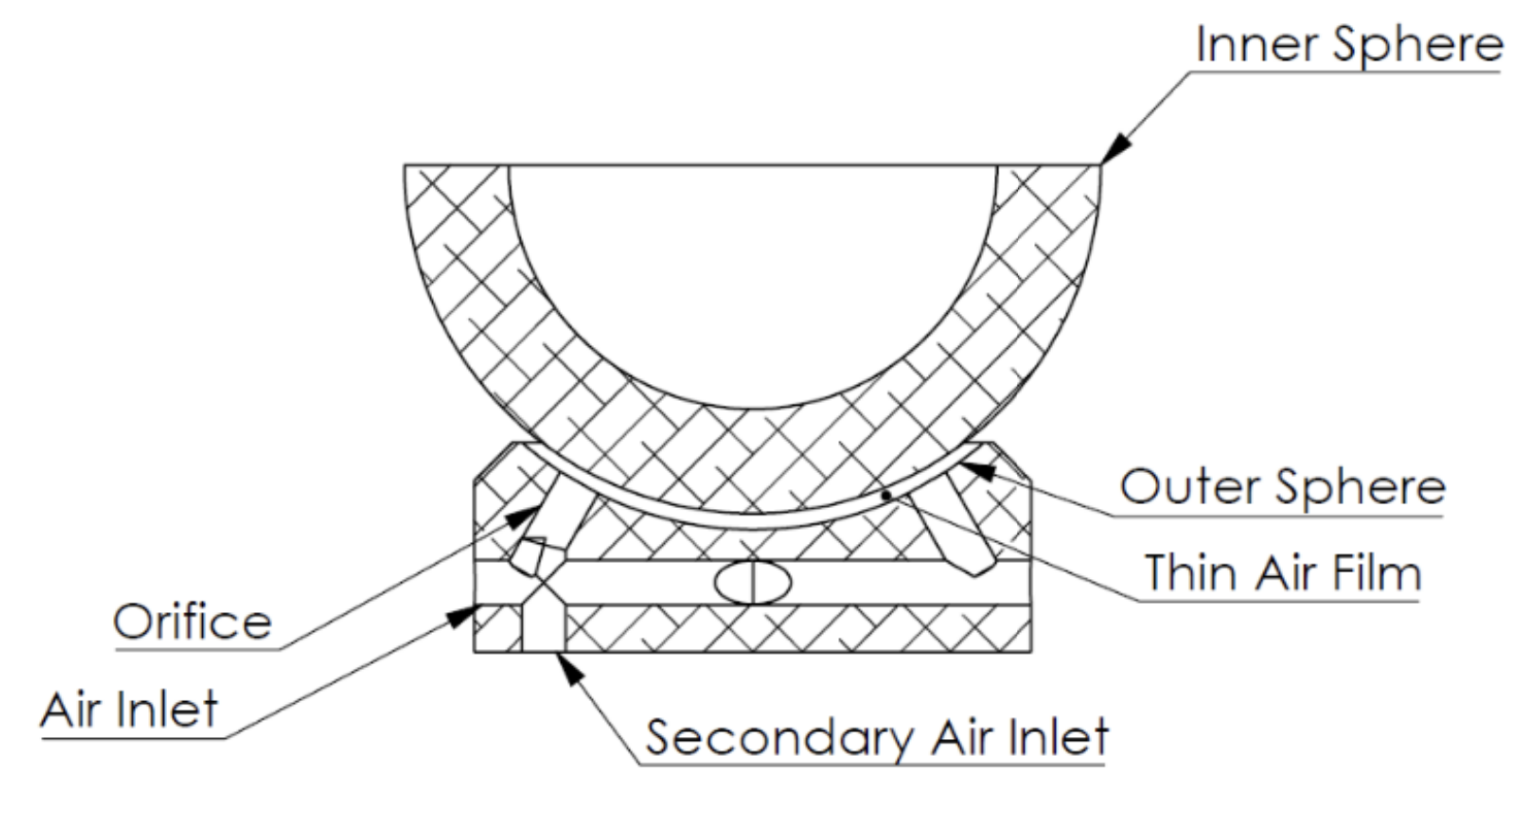
\includegraphics[width=0.70\linewidth]{figures/cross_section.png}
    \caption{A cross section of a spherical air bearing \cite{huang_characterizing_2022}}
    \label{fig:cross_section}
\end{figure}

The attitude determination and control system (ADCS) of a spacecraft is key subsystem that undergoes such a series of tests. A typical series is shown in \Cref{fig:ADCS_tests}. Spacecraft dynamics simulators represent any test apparatus that recreates the attiude dynamics seen on-orbit.  The two primary goals then are to provide frictionless, torque-free rotations. As seen in \Cref{fig:cross_section}, the most common method mounts the test hardware to a spherical air-bearing, allowing the platform to freely rotate about its yaw axis, and within some limited range about it's pitch and roll axes. From here the full suite of ADCS hardware may be integrated onto the platform, including sensors, a flight computer, and actuators. 

The thin layer of compressed between the spherical mount and platform ensures rotation with near-zero friction~\cite{huang_characterizing_2022}. However, while an air-bearing helps guarantee frictionless rotation, any distance between the platform's center of mass and it's center of rotation will introduce a torque due to gravity that is not seen in space. If this torque is large enough, even basic tasks like repointing may not be able to be performed on the simulator. To compensate for this simulator's shift their center of mass by changing the position of sliding masses onboard~\cite{kim_automatic_2009}. The end goal is to adjust the mass blocks' positions such that the mass distribution of the platform changes, and the distance between the platform's center of mass and center of rotation is minmized. These masses may be adjusted by hand with visual inspection (referred to as manual mass balancing), or they may be precisely controlled using a preset balancing algorithm and linear actuators (referred to as automatic mass balancing). The requirements of the balancing system is largely determined by the length of tests that are desired. Smaller torques due to gravity will allow the actuators exchange more momentum with the platform before saturating. 


\section{Thesis Overview}\label{sec:previous_work}

Research laboratories and universities take part in building their own dynamics simulators for educational purposes and as a way to test novel control algorithms and hardware. The Cal Poly Spacecraft Attitude Dynamics Simulator (SADS) is part of this category and has been developed by students and faculty since it's first introduction in 2007 \cite{mittelsteadt_cal_2007}. 

\begin{figure}[h]\label{fig:V1}
    \centering
    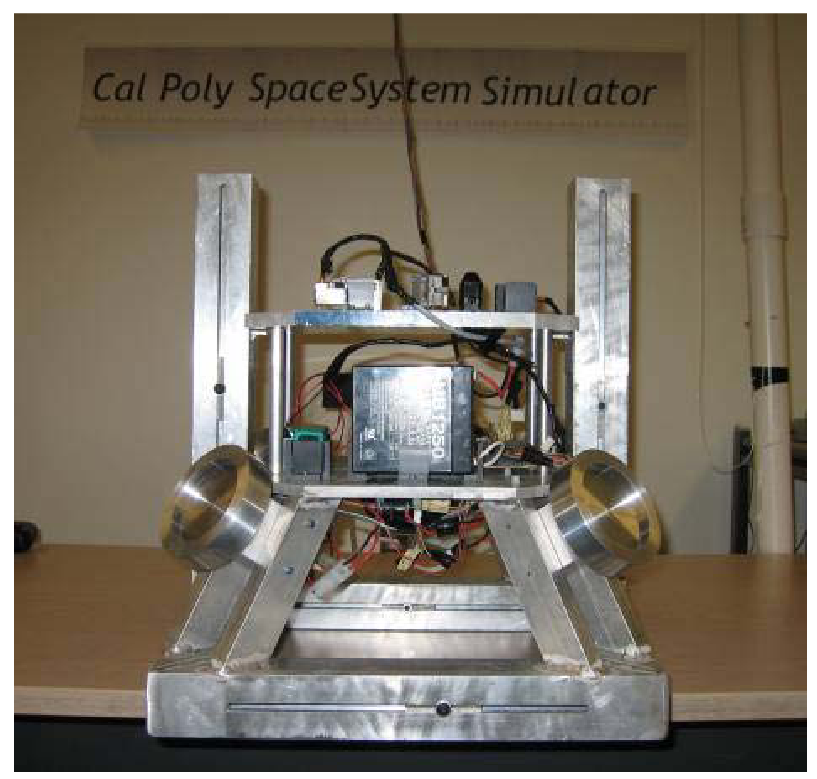
\includegraphics[width=0.80\linewidth]{figures/SADS_V1.PNG}
    \caption{The first iteration of the Cal Poly SADS \cite{mittelsteadt_cal_2007}}
\end{figure}

Beginning in 2023 an effort began to modernize the hardware on the SADS, which included the mass balancing system. This thesis contributes to that effort by advancing the overall design of the new SADS iteration and performing experimental tests of the newly designed and integrating mass balancing system. \Cref{chap:background} describes a historical overview of mass balancing systems and survey of the hardware and algorithms used on contemporary designs. It additionally provides a detailed history of the SADS and the evolution of it's own mass balancing system, after which the thesis objectives are formally stated. \Cref{chap:methodology} introduces the theoretical framework and conventions used to solve the balancing problem and the details of it's practical implementation on the SADS. \Cref{chap:results} discusses the results of the newly designed system in simulation and experiment and characterizes the achieved balancing results.



% The platform was first introduced in 2007~\cite{mittelsteadt_cal_2007} and featured a set mass blocks that slid along slots cut out from the structure. These blocks had to be adjusted by hand, and adjustments were made by observing the platforms inbalance visually and making incremental changes.

% In 2010, Silva attempted to improve on this method by using a least-squares estimation algorithm to estimate the center of mass. This requires taking body rate when the platform is tumbling under the influence of gravity. Unfortunately the measurement system at the time only could provide low-rate gyroscope data which significantly hindered the balancing results. Dam followed up on this in 2014 using a navigation-grade IMU to provide high-quality body rate data at 20 Hz. This significantly improved balancing results, with the final estimated center of mass after balancing being on the order of $10^{-3}$ meters.

% Beginning in 2023 an effort was made to modernize the hardware on the SADS, which included the MBS.\@ In 2024 Gilman worked on a set of custom linear actuators that could finely control the positions of sliding masses onboard. Due to a lack of a finished flight computer and measurement system, the actuators could only be tested in hardware-in-the-loop conditions. How these various mass balancing implementations compare against those found in literature will be discussed in depth in \Cref{chap:background}. 




